\documentclass[12pt]{article}

    %\usepackage[breakable]{tcolorbox}
    \usepackage[most]{tcolorbox}
    \usepackage{lmodern} 
    \usepackage{parskip} % Stop auto-indenting (to mimic markdown behaviour)
    
    \usepackage{iftex}
    \ifPDFTeX
    	\usepackage[T1]{fontenc}
    	\usepackage{mathpazo}
    \else
    	\usepackage{fontspec}
    \fi

    % Basic figure setup, for now with no caption control since it's done
    % automatically by Pandoc (which extracts ![](path) syntax from Markdown).
    \usepackage{graphicx}
    % Maintain compatibility with old templates. Remove in nbconvert 6.0
    \let\Oldincludegraphics\includegraphics
    % Ensure that by default, figures have no caption (until we provide a
    % proper Figure object with a Caption API and a way to capture that
    % in the conversion process - todo).
    \usepackage{caption}
    \DeclareCaptionFormat{nocaption}{}
    \captionsetup{format=nocaption,aboveskip=0pt,belowskip=0pt}

    \usepackage{float}
    \floatplacement{figure}{H} % forces figures to be placed at the correct location
    \usepackage{xcolor} % Allow colors to be defined
    \usepackage{enumerate} % Needed for markdown enumerations to work
    \usepackage{geometry} % Used to adjust the document margins
    \usepackage{amsmath} % Equations
    \usepackage{amssymb} % Equations
    \usepackage{textcomp} % defines textquotesingle
    % Hack from http://tex.stackexchange.com/a/47451/13684:
    \AtBeginDocument{%
        \def\PYZsq{\textquotesingle}% Upright quotes in Pygmentized code
    }
    \usepackage{upquote} % Upright quotes for verbatim code
    \usepackage{eurosym} % defines \euro
    \usepackage[mathletters]{ucs} % Extended unicode (utf-8) support
    \usepackage{fancyvrb} % verbatim replacement that allows latex
    \usepackage{grffile} % extends the file name processing of package graphics 
                         % to support a larger range
    \makeatletter % fix for old versions of grffile with XeLaTeX
    \@ifpackagelater{grffile}{2019/11/01}
    {
      % Do nothing on new versions
    }
    {
      \def\Gread@@xetex#1{%
        \IfFileExists{"\Gin@base".bb}%
        {\Gread@eps{\Gin@base.bb}}%
        {\Gread@@xetex@aux#1}%
      }
    }
    \makeatother
    \usepackage[Export]{adjustbox} % Used to constrain images to a maximum size
    \adjustboxset{max size={0.9\linewidth}{0.9\paperheight}}

    % The hyperref package gives us a pdf with properly built
    % internal navigation ('pdf bookmarks' for the table of contents,
    % internal cross-reference links, web links for URLs, etc.)
    \usepackage{hyperref}
    % The default LaTeX title has an obnoxious amount of whitespace. By default,
    % titling removes some of it. It also provides customization options.
    \usepackage{titling}
    \usepackage{longtable} % longtable support required by pandoc >1.10
    \usepackage{booktabs}  % table support for pandoc > 1.12.2
    \usepackage[inline]{enumitem} % IRkernel/repr support (it uses the enumerate* environment)
    \usepackage[normalem]{ulem} % ulem is needed to support strikethroughs (\sout)
                                % normalem makes italics be italics, not underlines
    \usepackage{mathrsfs}
    
\usepackage{fancyhdr}
\usepackage{lastpage}
\usepackage{cclicenses}

    % Colors for the hyperref package
    \definecolor{urlcolor}{rgb}{0,.145,.698}
    \definecolor{linkcolor}{rgb}{.71,0.21,0.01}
    \definecolor{citecolor}{rgb}{.12,.54,.11}

    % ANSI colors
    \definecolor{ansi-black}{HTML}{3E424D}
    \definecolor{ansi-black-intense}{HTML}{282C36}
    \definecolor{ansi-red}{HTML}{E75C58}
    \definecolor{ansi-red-intense}{HTML}{B22B31}
    \definecolor{ansi-green}{HTML}{00A250}
    \definecolor{ansi-green-intense}{HTML}{007427}
    \definecolor{ansi-yellow}{HTML}{DDB62B}
    \definecolor{ansi-yellow-intense}{HTML}{B27D12}
    \definecolor{ansi-blue}{HTML}{208FFB}
    \definecolor{ansi-blue-intense}{HTML}{0065CA}
    \definecolor{ansi-magenta}{HTML}{D160C4}
    \definecolor{ansi-magenta-intense}{HTML}{A03196}
    \definecolor{ansi-cyan}{HTML}{60C6C8}
    \definecolor{ansi-cyan-intense}{HTML}{258F8F}
    \definecolor{ansi-white}{HTML}{C5C1B4}
    \definecolor{ansi-white-intense}{HTML}{A1A6B2}
    \definecolor{ansi-default-inverse-fg}{HTML}{FFFFFF}
    \definecolor{ansi-default-inverse-bg}{HTML}{000000}

    % common color for the border for error outputs.
    \definecolor{outerrorbackground}{HTML}{FFDFDF}

    % commands and environments needed by pandoc snippets
    % extracted from the output of `pandoc -s`
    \providecommand{\tightlist}{%
      \setlength{\itemsep}{0pt}\setlength{\parskip}{0pt}}
    \DefineVerbatimEnvironment{Highlighting}{Verbatim}{commandchars=\\\{\}}
    % Add ',fontsize=\small' for more characters per line
    \newenvironment{Shaded}{}{}
    \newcommand{\KeywordTok}[1]{\textcolor[rgb]{0.00,0.44,0.13}{\textbf{{#1}}}}
    \newcommand{\DataTypeTok}[1]{\textcolor[rgb]{0.56,0.13,0.00}{{#1}}}
    \newcommand{\DecValTok}[1]{\textcolor[rgb]{0.25,0.63,0.44}{{#1}}}
    \newcommand{\BaseNTok}[1]{\textcolor[rgb]{0.25,0.63,0.44}{{#1}}}
    \newcommand{\FloatTok}[1]{\textcolor[rgb]{0.25,0.63,0.44}{{#1}}}
    \newcommand{\CharTok}[1]{\textcolor[rgb]{0.25,0.44,0.63}{{#1}}}
    \newcommand{\StringTok}[1]{\textcolor[rgb]{0.25,0.44,0.63}{{#1}}}
    \newcommand{\CommentTok}[1]{\textcolor[rgb]{0.38,0.63,0.69}{\textit{{#1}}}}
    \newcommand{\OtherTok}[1]{\textcolor[rgb]{0.00,0.44,0.13}{{#1}}}
    \newcommand{\AlertTok}[1]{\textcolor[rgb]{1.00,0.00,0.00}{\textbf{{#1}}}}
    \newcommand{\FunctionTok}[1]{\textcolor[rgb]{0.02,0.16,0.49}{{#1}}}
    \newcommand{\RegionMarkerTok}[1]{{#1}}
    \newcommand{\ErrorTok}[1]{\textcolor[rgb]{1.00,0.00,0.00}{\textbf{{#1}}}}
    \newcommand{\NormalTok}[1]{{#1}}
    
    % Additional commands for more recent versions of Pandoc
    \newcommand{\ConstantTok}[1]{\textcolor[rgb]{0.53,0.00,0.00}{{#1}}}
    \newcommand{\SpecialCharTok}[1]{\textcolor[rgb]{0.25,0.44,0.63}{{#1}}}
    \newcommand{\VerbatimStringTok}[1]{\textcolor[rgb]{0.25,0.44,0.63}{{#1}}}
    \newcommand{\SpecialStringTok}[1]{\textcolor[rgb]{0.73,0.40,0.53}{{#1}}}
    \newcommand{\ImportTok}[1]{{#1}}
    \newcommand{\DocumentationTok}[1]{\textcolor[rgb]{0.73,0.13,0.13}{\textit{{#1}}}}
    \newcommand{\AnnotationTok}[1]{\textcolor[rgb]{0.38,0.63,0.69}{\textbf{\textit{{#1}}}}}
    \newcommand{\CommentVarTok}[1]{\textcolor[rgb]{0.38,0.63,0.69}{\textbf{\textit{{#1}}}}}
    \newcommand{\VariableTok}[1]{\textcolor[rgb]{0.10,0.09,0.49}{{#1}}}
    \newcommand{\ControlFlowTok}[1]{\textcolor[rgb]{0.00,0.44,0.13}{\textbf{{#1}}}}
    \newcommand{\OperatorTok}[1]{\textcolor[rgb]{0.40,0.40,0.40}{{#1}}}
    \newcommand{\BuiltInTok}[1]{{#1}}
    \newcommand{\ExtensionTok}[1]{{#1}}
    \newcommand{\PreprocessorTok}[1]{\textcolor[rgb]{0.74,0.48,0.00}{{#1}}}
    \newcommand{\AttributeTok}[1]{\textcolor[rgb]{0.49,0.56,0.16}{{#1}}}
    \newcommand{\InformationTok}[1]{\textcolor[rgb]{0.38,0.63,0.69}{\textbf{\textit{{#1}}}}}
    \newcommand{\WarningTok}[1]{\textcolor[rgb]{0.38,0.63,0.69}{\textbf{\textit{{#1}}}}}
    
    % Slightly bigger margins than the latex defaults
    
    \geometry{verbose,tmargin=0.7in,bmargin=0.7in,lmargin=0.7in,rmargin=0.7in}
        
    % Define a nice break command that doesn't care if a line doesn't already
    % exist.
    \def\br{\hspace*{\fill} \\* }
    % Math Jax compatibility definitions
    \def\gt{>}
    \def\lt{<}
    \let\Oldtex\TeX
    \let\Oldlatex\LaTeX
    \renewcommand{\TeX}{\textrm{\Oldtex}}
    \renewcommand{\LaTeX}{\textrm{\Oldlatex}}
    % Document parameters
    % Document title
    \title{Opérateurs logiques}
      \date{Octobre 2021}  
	%\author{Yannick Chistel}
    
\makeatletter         
\renewcommand\maketitle[1]{
\hrule\medskip
{\raggedright % Note the extra {
\begin{center}
{\Huge \bfseries \sffamily #1 }\\[4ex] 
%{\Large  \@author}\\[2ex] 
%\@date\\[4ex]
\hrule \bigskip
\end{center}}} % Note the extra }
\makeatother    



\pagestyle{fancy}
\fancyhead{}
\renewcommand\headrulewidth{0pt}
\renewcommand\footrulewidth{1pt}
\fancyfoot[L]{YC}
\fancyfoot[C]{\thepage}
\fancyfoot[R]{\cc-\ccby-\ccnc}

% 
%\newtcolorbox{exemple}[2][]{
%    enhanced,
%    size=fbox,sharp corners,
%    colback=white,colframe=black,
%    colbacktitle=black,fonttitle=\bfseries,
%    attach boxed title to top left={yshift=-3mm,yshifttext=-3mm},
%    boxed title style={size=small,left=0pt,right=0pt,sharp corners},title=#2,#1}

\newtcolorbox{remarque}[2][]{colback=red!4!white,
colframe=red!64!black,fonttitle=\bfseries,
colbacktitle=red!64!black,enhanced,
attach boxed title to top left={xshift=4mm,yshift=-2mm},
title=#2,#1}  


\newtcolorbox{exemple}[2][]{colback=blue!4!white,
colframe=blue!64!green,fonttitle=\bfseries,
colbacktitle=blue!64!green,enhanced,
attach boxed title to top left={xshift=4mm,yshift=-2mm},
title=#2,#1}  
    
% Pygments definitions
\makeatletter
\def\PY@reset{\let\PY@it=\relax \let\PY@bf=\relax%
    \let\PY@ul=\relax \let\PY@tc=\relax%
    \let\PY@bc=\relax \let\PY@ff=\relax}
\def\PY@tok#1{\csname PY@tok@#1\endcsname}
\def\PY@toks#1+{\ifx\relax#1\empty\else%
    \PY@tok{#1}\expandafter\PY@toks\fi}
\def\PY@do#1{\PY@bc{\PY@tc{\PY@ul{%
    \PY@it{\PY@bf{\PY@ff{#1}}}}}}}
\def\PY#1#2{\PY@reset\PY@toks#1+\relax+\PY@do{#2}}

\@namedef{PY@tok@w}{\def\PY@tc##1{\textcolor[rgb]{0.73,0.73,0.73}{##1}}}
\@namedef{PY@tok@c}{\let\PY@it=\textit\def\PY@tc##1{\textcolor[rgb]{0.25,0.50,0.50}{##1}}}
\@namedef{PY@tok@cp}{\def\PY@tc##1{\textcolor[rgb]{0.74,0.48,0.00}{##1}}}
\@namedef{PY@tok@k}{\let\PY@bf=\textbf\def\PY@tc##1{\textcolor[rgb]{0.00,0.50,0.00}{##1}}}
\@namedef{PY@tok@kp}{\def\PY@tc##1{\textcolor[rgb]{0.00,0.50,0.00}{##1}}}
\@namedef{PY@tok@kt}{\def\PY@tc##1{\textcolor[rgb]{0.69,0.00,0.25}{##1}}}
\@namedef{PY@tok@o}{\def\PY@tc##1{\textcolor[rgb]{0.40,0.40,0.40}{##1}}}
\@namedef{PY@tok@ow}{\let\PY@bf=\textbf\def\PY@tc##1{\textcolor[rgb]{0.67,0.13,1.00}{##1}}}
\@namedef{PY@tok@nb}{\def\PY@tc##1{\textcolor[rgb]{0.00,0.50,0.00}{##1}}}
\@namedef{PY@tok@nf}{\def\PY@tc##1{\textcolor[rgb]{0.00,0.00,1.00}{##1}}}
\@namedef{PY@tok@nc}{\let\PY@bf=\textbf\def\PY@tc##1{\textcolor[rgb]{0.00,0.00,1.00}{##1}}}
\@namedef{PY@tok@nn}{\let\PY@bf=\textbf\def\PY@tc##1{\textcolor[rgb]{0.00,0.00,1.00}{##1}}}
\@namedef{PY@tok@ne}{\let\PY@bf=\textbf\def\PY@tc##1{\textcolor[rgb]{0.82,0.25,0.23}{##1}}}
\@namedef{PY@tok@nv}{\def\PY@tc##1{\textcolor[rgb]{0.10,0.09,0.49}{##1}}}
\@namedef{PY@tok@no}{\def\PY@tc##1{\textcolor[rgb]{0.53,0.00,0.00}{##1}}}
\@namedef{PY@tok@nl}{\def\PY@tc##1{\textcolor[rgb]{0.63,0.63,0.00}{##1}}}
\@namedef{PY@tok@ni}{\let\PY@bf=\textbf\def\PY@tc##1{\textcolor[rgb]{0.60,0.60,0.60}{##1}}}
\@namedef{PY@tok@na}{\def\PY@tc##1{\textcolor[rgb]{0.49,0.56,0.16}{##1}}}
\@namedef{PY@tok@nt}{\let\PY@bf=\textbf\def\PY@tc##1{\textcolor[rgb]{0.00,0.50,0.00}{##1}}}
\@namedef{PY@tok@nd}{\def\PY@tc##1{\textcolor[rgb]{0.67,0.13,1.00}{##1}}}
\@namedef{PY@tok@s}{\def\PY@tc##1{\textcolor[rgb]{0.73,0.13,0.13}{##1}}}
\@namedef{PY@tok@sd}{\let\PY@it=\textit\def\PY@tc##1{\textcolor[rgb]{0.73,0.13,0.13}{##1}}}
\@namedef{PY@tok@si}{\let\PY@bf=\textbf\def\PY@tc##1{\textcolor[rgb]{0.73,0.40,0.53}{##1}}}
\@namedef{PY@tok@se}{\let\PY@bf=\textbf\def\PY@tc##1{\textcolor[rgb]{0.73,0.40,0.13}{##1}}}
\@namedef{PY@tok@sr}{\def\PY@tc##1{\textcolor[rgb]{0.73,0.40,0.53}{##1}}}
\@namedef{PY@tok@ss}{\def\PY@tc##1{\textcolor[rgb]{0.10,0.09,0.49}{##1}}}
\@namedef{PY@tok@sx}{\def\PY@tc##1{\textcolor[rgb]{0.00,0.50,0.00}{##1}}}
\@namedef{PY@tok@m}{\def\PY@tc##1{\textcolor[rgb]{0.40,0.40,0.40}{##1}}}
\@namedef{PY@tok@gh}{\let\PY@bf=\textbf\def\PY@tc##1{\textcolor[rgb]{0.00,0.00,0.50}{##1}}}
\@namedef{PY@tok@gu}{\let\PY@bf=\textbf\def\PY@tc##1{\textcolor[rgb]{0.50,0.00,0.50}{##1}}}
\@namedef{PY@tok@gd}{\def\PY@tc##1{\textcolor[rgb]{0.63,0.00,0.00}{##1}}}
\@namedef{PY@tok@gi}{\def\PY@tc##1{\textcolor[rgb]{0.00,0.63,0.00}{##1}}}
\@namedef{PY@tok@gr}{\def\PY@tc##1{\textcolor[rgb]{1.00,0.00,0.00}{##1}}}
\@namedef{PY@tok@ge}{\let\PY@it=\textit}
\@namedef{PY@tok@gs}{\let\PY@bf=\textbf}
\@namedef{PY@tok@gp}{\let\PY@bf=\textbf\def\PY@tc##1{\textcolor[rgb]{0.00,0.00,0.50}{##1}}}
\@namedef{PY@tok@go}{\def\PY@tc##1{\textcolor[rgb]{0.53,0.53,0.53}{##1}}}
\@namedef{PY@tok@gt}{\def\PY@tc##1{\textcolor[rgb]{0.00,0.27,0.87}{##1}}}
\@namedef{PY@tok@err}{\def\PY@bc##1{{\setlength{\fboxsep}{\string -\fboxrule}\fcolorbox[rgb]{1.00,0.00,0.00}{1,1,1}{\strut ##1}}}}
\@namedef{PY@tok@kc}{\let\PY@bf=\textbf\def\PY@tc##1{\textcolor[rgb]{0.00,0.50,0.00}{##1}}}
\@namedef{PY@tok@kd}{\let\PY@bf=\textbf\def\PY@tc##1{\textcolor[rgb]{0.00,0.50,0.00}{##1}}}
\@namedef{PY@tok@kn}{\let\PY@bf=\textbf\def\PY@tc##1{\textcolor[rgb]{0.00,0.50,0.00}{##1}}}
\@namedef{PY@tok@kr}{\let\PY@bf=\textbf\def\PY@tc##1{\textcolor[rgb]{0.00,0.50,0.00}{##1}}}
\@namedef{PY@tok@bp}{\def\PY@tc##1{\textcolor[rgb]{0.00,0.50,0.00}{##1}}}
\@namedef{PY@tok@fm}{\def\PY@tc##1{\textcolor[rgb]{0.00,0.00,1.00}{##1}}}
\@namedef{PY@tok@vc}{\def\PY@tc##1{\textcolor[rgb]{0.10,0.09,0.49}{##1}}}
\@namedef{PY@tok@vg}{\def\PY@tc##1{\textcolor[rgb]{0.10,0.09,0.49}{##1}}}
\@namedef{PY@tok@vi}{\def\PY@tc##1{\textcolor[rgb]{0.10,0.09,0.49}{##1}}}
\@namedef{PY@tok@vm}{\def\PY@tc##1{\textcolor[rgb]{0.10,0.09,0.49}{##1}}}
\@namedef{PY@tok@sa}{\def\PY@tc##1{\textcolor[rgb]{0.73,0.13,0.13}{##1}}}
\@namedef{PY@tok@sb}{\def\PY@tc##1{\textcolor[rgb]{0.73,0.13,0.13}{##1}}}
\@namedef{PY@tok@sc}{\def\PY@tc##1{\textcolor[rgb]{0.73,0.13,0.13}{##1}}}
\@namedef{PY@tok@dl}{\def\PY@tc##1{\textcolor[rgb]{0.73,0.13,0.13}{##1}}}
\@namedef{PY@tok@s2}{\def\PY@tc##1{\textcolor[rgb]{0.73,0.13,0.13}{##1}}}
\@namedef{PY@tok@sh}{\def\PY@tc##1{\textcolor[rgb]{0.73,0.13,0.13}{##1}}}
\@namedef{PY@tok@s1}{\def\PY@tc##1{\textcolor[rgb]{0.73,0.13,0.13}{##1}}}
\@namedef{PY@tok@mb}{\def\PY@tc##1{\textcolor[rgb]{0.40,0.40,0.40}{##1}}}
\@namedef{PY@tok@mf}{\def\PY@tc##1{\textcolor[rgb]{0.40,0.40,0.40}{##1}}}
\@namedef{PY@tok@mh}{\def\PY@tc##1{\textcolor[rgb]{0.40,0.40,0.40}{##1}}}
\@namedef{PY@tok@mi}{\def\PY@tc##1{\textcolor[rgb]{0.40,0.40,0.40}{##1}}}
\@namedef{PY@tok@il}{\def\PY@tc##1{\textcolor[rgb]{0.40,0.40,0.40}{##1}}}
\@namedef{PY@tok@mo}{\def\PY@tc##1{\textcolor[rgb]{0.40,0.40,0.40}{##1}}}
\@namedef{PY@tok@ch}{\let\PY@it=\textit\def\PY@tc##1{\textcolor[rgb]{0.25,0.50,0.50}{##1}}}
\@namedef{PY@tok@cm}{\let\PY@it=\textit\def\PY@tc##1{\textcolor[rgb]{0.25,0.50,0.50}{##1}}}
\@namedef{PY@tok@cpf}{\let\PY@it=\textit\def\PY@tc##1{\textcolor[rgb]{0.25,0.50,0.50}{##1}}}
\@namedef{PY@tok@c1}{\let\PY@it=\textit\def\PY@tc##1{\textcolor[rgb]{0.25,0.50,0.50}{##1}}}
\@namedef{PY@tok@cs}{\let\PY@it=\textit\def\PY@tc##1{\textcolor[rgb]{0.25,0.50,0.50}{##1}}}

\def\PYZbs{\char`\\}
\def\PYZus{\char`\_}
\def\PYZob{\char`\{}
\def\PYZcb{\char`\}}
\def\PYZca{\char`\^}
\def\PYZam{\char`\&}
\def\PYZlt{\char`\<}
\def\PYZgt{\char`\>}
\def\PYZsh{\char`\#}
\def\PYZpc{\char`\%}
\def\PYZdl{\char`\$}
\def\PYZhy{\char`\-}
\def\PYZsq{\char`\'}
\def\PYZdq{\char`\"}
\def\PYZti{\char`\~}
% for compatibility with earlier versions
\def\PYZat{@}
\def\PYZlb{[}
\def\PYZrb{]}
\makeatother


    % For linebreaks inside Verbatim environment from package fancyvrb. 
    \makeatletter
        \newbox\Wrappedcontinuationbox 
        \newbox\Wrappedvisiblespacebox 
        \newcommand*\Wrappedvisiblespace {\textcolor{red}{\textvisiblespace}} 
        \newcommand*\Wrappedcontinuationsymbol {\textcolor{red}{\llap{\tiny$\m@th\hookrightarrow$}}} 
        \newcommand*\Wrappedcontinuationindent {3ex } 
        \newcommand*\Wrappedafterbreak {\kern\Wrappedcontinuationindent\copy\Wrappedcontinuationbox} 
        % Take advantage of the already applied Pygments mark-up to insert 
        % potential linebreaks for TeX processing. 
        %        {, <, #, %, $, ' and ": go to next line. 
        %        _, }, ^, &, >, - and ~: stay at end of broken line. 
        % Use of \textquotesingle for straight quote. 
        \newcommand*\Wrappedbreaksatspecials {% 
            \def\PYGZus{\discretionary{\char`\_}{\Wrappedafterbreak}{\char`\_}}% 
            \def\PYGZob{\discretionary{}{\Wrappedafterbreak\char`\{}{\char`\{}}% 
            \def\PYGZcb{\discretionary{\char`\}}{\Wrappedafterbreak}{\char`\}}}% 
            \def\PYGZca{\discretionary{\char`\^}{\Wrappedafterbreak}{\char`\^}}% 
            \def\PYGZam{\discretionary{\char`\&}{\Wrappedafterbreak}{\char`\&}}% 
            \def\PYGZlt{\discretionary{}{\Wrappedafterbreak\char`\<}{\char`\<}}% 
            \def\PYGZgt{\discretionary{\char`\>}{\Wrappedafterbreak}{\char`\>}}% 
            \def\PYGZsh{\discretionary{}{\Wrappedafterbreak\char`\#}{\char`\#}}% 
            \def\PYGZpc{\discretionary{}{\Wrappedafterbreak\char`\%}{\char`\%}}% 
            \def\PYGZdl{\discretionary{}{\Wrappedafterbreak\char`\$}{\char`\$}}% 
            \def\PYGZhy{\discretionary{\char`\-}{\Wrappedafterbreak}{\char`\-}}% 
            \def\PYGZsq{\discretionary{}{\Wrappedafterbreak\textquotesingle}{\textquotesingle}}% 
            \def\PYGZdq{\discretionary{}{\Wrappedafterbreak\char`\"}{\char`\"}}% 
            \def\PYGZti{\discretionary{\char`\~}{\Wrappedafterbreak}{\char`\~}}% 
        } 
        % Some characters . , ; ? ! / are not pygmentized. 
        % This macro makes them "active" and they will insert potential linebreaks 
        \newcommand*\Wrappedbreaksatpunct {% 
            \lccode`\~`\.\lowercase{\def~}{\discretionary{\hbox{\char`\.}}{\Wrappedafterbreak}{\hbox{\char`\.}}}% 
            \lccode`\~`\,\lowercase{\def~}{\discretionary{\hbox{\char`\,}}{\Wrappedafterbreak}{\hbox{\char`\,}}}% 
            \lccode`\~`\;\lowercase{\def~}{\discretionary{\hbox{\char`\;}}{\Wrappedafterbreak}{\hbox{\char`\;}}}% 
            \lccode`\~`\:\lowercase{\def~}{\discretionary{\hbox{\char`\:}}{\Wrappedafterbreak}{\hbox{\char`\:}}}% 
            \lccode`\~`\?\lowercase{\def~}{\discretionary{\hbox{\char`\?}}{\Wrappedafterbreak}{\hbox{\char`\?}}}% 
            \lccode`\~`\!\lowercase{\def~}{\discretionary{\hbox{\char`\!}}{\Wrappedafterbreak}{\hbox{\char`\!}}}% 
            \lccode`\~`\/\lowercase{\def~}{\discretionary{\hbox{\char`\/}}{\Wrappedafterbreak}{\hbox{\char`\/}}}% 
            \catcode`\.\active
            \catcode`\,\active 
            \catcode`\;\active
            \catcode`\:\active
            \catcode`\?\active
            \catcode`\!\active
            \catcode`\/\active 
            \lccode`\~`\~ 	
        }
    \makeatother

    \let\OriginalVerbatim=\Verbatim
    \makeatletter
    \renewcommand{\Verbatim}[1][1]{%
        %\parskip\z@skip
        \sbox\Wrappedcontinuationbox {\Wrappedcontinuationsymbol}%
        \sbox\Wrappedvisiblespacebox {\FV@SetupFont\Wrappedvisiblespace}%
        \def\FancyVerbFormatLine ##1{\hsize\linewidth
            \vtop{\raggedright\hyphenpenalty\z@\exhyphenpenalty\z@
                \doublehyphendemerits\z@\finalhyphendemerits\z@
                \strut ##1\strut}%
        }%
        % If the linebreak is at a space, the latter will be displayed as visible
        % space at end of first line, and a continuation symbol starts next line.
        % Stretch/shrink are however usually zero for typewriter font.
        \def\FV@Space {%
            \nobreak\hskip\z@ plus\fontdimen3\font minus\fontdimen4\font
            \discretionary{\copy\Wrappedvisiblespacebox}{\Wrappedafterbreak}
            {\kern\fontdimen2\font}%
        }%
        
        % Allow breaks at special characters using \PYG... macros.
        \Wrappedbreaksatspecials
        % Breaks at punctuation characters . , ; ? ! and / need catcode=\active 	
        \OriginalVerbatim[#1,codes*=\Wrappedbreaksatpunct]%
    }
    \makeatother

    % Exact colors from NB
    \definecolor{incolor}{HTML}{303F9F}
    \definecolor{outcolor}{HTML}{D84315}
    \definecolor{cellborder}{HTML}{CFCFCF}
    \definecolor{cellbackground}{HTML}{F7F7F7}
    
    % prompt
    \makeatletter
    \newcommand{\boxspacing}{\kern\kvtcb@left@rule\kern\kvtcb@boxsep}
    \makeatother
    \newcommand{\prompt}[4]{
        {\ttfamily\llap{{\color{#2}[#3]:\hspace{3pt}#4}}\vspace{-\baselineskip}}
    }
    

    
    % Prevent overflowing lines due to hard-to-break entities
    \sloppy 
    % Setup hyperref package
    \hypersetup{
      breaklinks=true,  % so long urls are correctly broken across lines
      colorlinks=true,
      urlcolor=urlcolor,
      linkcolor=linkcolor,
      citecolor=citecolor,
      }

    


\begin{document}
    
    \maketitle{Récursivité}
    

    
%    \hypertarget{exercices}{%
%\section{Exercices}\label{exercices}}

%    \hypertarget{fonctions-ruxe9cursives}{%
%\section{Fonctions récursives}\label{fonctions-ruxe9cursives}}

\hypertarget{exercice}{%
\subsection*{Exercice}\label{exercice}}

\begin{enumerate}
\def\labelenumi{\arabic{enumi}.}
\item
  La fonction ordre est récursive car la fonction s'appelle elle-même.\\
  Le cas de base est pour \(n=0\), provoquant l'arrêt des appels
  récursifs et qui renvoie la valeur `0' pour l'appel \texttt{ordre(0)}.
\item
  L'appel \texttt{ordre(4)} renvoie la chaine de caractères `01234'.
\item
  Si on intervertit dans la concaténation l'appel récursif et str(n),
  cela affiche les valeurs de \(n\) au début de la chaine de caractères
  dans un ordre décroissant.
\end{enumerate}

    \begin{tcolorbox}[breakable, size=fbox, boxrule=1pt, pad at break*=1mm,colback=cellbackground, colframe=cellborder]
\prompt{In}{incolor}{43}{\boxspacing}
\begin{Verbatim}[commandchars=\\\{\}]
\PY{c+c1}{\PYZsh{} Fonction récursive ordre}
\PY{k}{def} \PY{n+nf}{ordre}\PY{p}{(}\PY{n}{n}\PY{p}{)}\PY{p}{:}
    \PY{k}{if} \PY{n}{n} \PY{o}{==} \PY{l+m+mi}{0}\PY{p}{:}
        \PY{k}{return} \PY{l+s+s1}{\PYZsq{}}\PY{l+s+s1}{0}\PY{l+s+s1}{\PYZsq{}} 
    \PY{k}{else}\PY{p}{:}
        \PY{k}{return} \PY{n}{ordre}\PY{p}{(}\PY{n}{n}\PY{o}{\PYZhy{}}\PY{l+m+mi}{1}\PY{p}{)}\PY{o}{+}\PY{n+nb}{str}\PY{p}{(}\PY{n}{n}\PY{p}{)}
    
\PY{n+nb}{print}\PY{p}{(}\PY{n}{ordre}\PY{p}{(}\PY{l+m+mi}{4}\PY{p}{)}\PY{p}{)}
\end{Verbatim}
\end{tcolorbox}

    \begin{Verbatim}[commandchars=\\\{\}]
01234
    \end{Verbatim}

    \begin{tcolorbox}[breakable, size=fbox, boxrule=1pt, pad at break*=1mm,colback=cellbackground, colframe=cellborder]
\prompt{In}{incolor}{44}{\boxspacing}
\begin{Verbatim}[commandchars=\\\{\}]
\PY{c+c1}{\PYZsh{} Fonction récursive ordre}
\PY{k}{def} \PY{n+nf}{ordre}\PY{p}{(}\PY{n}{n}\PY{p}{)}\PY{p}{:}
    \PY{k}{if} \PY{n}{n} \PY{o}{==} \PY{l+m+mi}{0}\PY{p}{:}
        \PY{k}{return} \PY{l+s+s1}{\PYZsq{}}\PY{l+s+s1}{0}\PY{l+s+s1}{\PYZsq{}} 
    \PY{k}{else}\PY{p}{:}
        \PY{k}{return} \PY{n+nb}{str}\PY{p}{(}\PY{n}{n}\PY{p}{)}\PY{o}{+}\PY{n}{ordre}\PY{p}{(}\PY{n}{n}\PY{o}{\PYZhy{}}\PY{l+m+mi}{1}\PY{p}{)}
    
\PY{n+nb}{print}\PY{p}{(}\PY{n}{ordre}\PY{p}{(}\PY{l+m+mi}{4}\PY{p}{)}\PY{p}{)}
\end{Verbatim}
\end{tcolorbox}

    \begin{Verbatim}[commandchars=\\\{\}]
43210
    \end{Verbatim}

    \hypertarget{exercice}{%
\subsection*{Exercice}\label{exercice}}

\begin{enumerate}
\def\labelenumi{\arabic{enumi}.}
\item
  La fonction \textbf{compte} est récursive car elle s'appelle
  elle-même.\\
  Le cas de base est pour \(n=1\) arrêtant les appels récursifs et
  renvoyant la valeur 1 pour l'appel \texttt{compte(1)}.
\item
  L'appel \texttt{compte(5)} renvoie la valeur 5 puisqu'on ajoute 1 à
  chaque appel récursif au nombre de 5.
\item
  Si on remplace la dernière instruction par
  \texttt{return\ 1+compte(n-2)}, on a deux cas différents:
\end{enumerate}

\begin{itemize}
\tightlist
\item
  si n est impair, alors \(n-2\) est toujours impair et finit par être
  égal à 1, arrêtant la récursivité et renvoyant la valeur 1 à l'appel
  \texttt{compte(1)}. Au final, on a compté les valeurs impaires soit
  \((n+1)/2\);
\item
  si n est pair, alors \(n-2\) est toujours pair et n'est donc jamais
  égal à 1. Les appels récursifs ne s'arrêtent pas provoquant une erreur
  de type \textbf{RecursionError: maximum recursion depth exceeded in
  comparison} soit trop d'appels récursifs. Le cas de base n'est jamais
  réalisé.
\end{itemize}

    \begin{tcolorbox}[breakable, size=fbox, boxrule=1pt, pad at break*=1mm,colback=cellbackground, colframe=cellborder]
\prompt{In}{incolor}{1}{\boxspacing}
\begin{Verbatim}[commandchars=\\\{\}]
\PY{c+c1}{\PYZsh{} Fonction récursive compte}
\PY{k}{def} \PY{n+nf}{compte}\PY{p}{(}\PY{n}{n}\PY{p}{)}\PY{p}{:}
    \PY{k}{if} \PY{n}{n} \PY{o}{==} \PY{l+m+mi}{1}\PY{p}{:}
        \PY{k}{return} \PY{l+m+mi}{1} 
    \PY{k}{else}\PY{p}{:}
        \PY{k}{return} \PY{l+m+mi}{1} \PY{o}{+} \PY{n}{compte}\PY{p}{(}\PY{n}{n}\PY{o}{\PYZhy{}}\PY{l+m+mi}{1}\PY{p}{)}
    
\PY{n+nb}{print}\PY{p}{(}\PY{n}{compte}\PY{p}{(}\PY{l+m+mi}{5}\PY{p}{)}\PY{p}{)}
\end{Verbatim}
\end{tcolorbox}

    \begin{Verbatim}[commandchars=\\\{\}]
5
    \end{Verbatim}

    \begin{tcolorbox}[breakable, size=fbox, boxrule=1pt, pad at break*=1mm,colback=cellbackground, colframe=cellborder]
\prompt{In}{incolor}{2}{\boxspacing}
\begin{Verbatim}[commandchars=\\\{\}]
\PY{c+c1}{\PYZsh{} Fonction récursive compte}
\PY{c+c1}{\PYZsh{} Une erreur est provoquée si n est pair !}
\PY{k}{def} \PY{n+nf}{compte}\PY{p}{(}\PY{n}{n}\PY{p}{)}\PY{p}{:}
    \PY{k}{if} \PY{n}{n} \PY{o}{==} \PY{l+m+mi}{1}\PY{p}{:}
        \PY{k}{return} \PY{l+m+mi}{1} 
    \PY{k}{else}\PY{p}{:}
        \PY{k}{return} \PY{l+m+mi}{1}\PY{o}{+}\PY{n}{compte}\PY{p}{(}\PY{n}{n}\PY{o}{\PYZhy{}}\PY{l+m+mi}{2}\PY{p}{)}
    
\PY{n+nb}{print}\PY{p}{(}\PY{n}{compte}\PY{p}{(}\PY{l+m+mi}{5}\PY{p}{)}\PY{p}{)}
\end{Verbatim}
\end{tcolorbox}

    \begin{Verbatim}[commandchars=\\\{\}]
3
    \end{Verbatim}

    \hypertarget{exercice}{%
\subsection*{Exercice}\label{exercice}}

\begin{enumerate}
\def\labelenumi{\arabic{enumi}.}
\tightlist
\item
  La commande \textbf{chr(65)} renvoie le caractère associé à la valeur
  décimale 65. Or \(65_{10}=41_{16}\) car \(4 \times 16 +1 = 65\).\\
  Dans la table ASCII, le caractère codé en hexadécimal \(41\) est la
  lettre majuscule \textbf{A}.
\item
  La boucle du script récupère les 26 lettres majuscules de l'alphabet
  et crée la chaine de caractères `ABCDEFGHIJKLMNOPQRSTUVWXYZ' qui est
  affichée avec la fonction \textbf{print}.
\item
  La version récursive est proposée ci-après.
\end{enumerate}

    \begin{tcolorbox}[breakable, size=fbox, boxrule=1pt, pad at break*=1mm,colback=cellbackground, colframe=cellborder]
\prompt{In}{incolor}{4}{\boxspacing}
\begin{Verbatim}[commandchars=\\\{\}]
\PY{c+c1}{\PYZsh{} Version itérative}
\PY{n}{mot}\PY{o}{=}\PY{l+s+s1}{\PYZsq{}}\PY{l+s+s1}{\PYZsq{}}
\PY{k}{for} \PY{n}{i} \PY{o+ow}{in} \PY{n+nb}{range}\PY{p}{(}\PY{l+m+mi}{65}\PY{p}{,}\PY{l+m+mi}{91}\PY{p}{)}\PY{p}{:} \PY{c+c1}{\PYZsh{} ou range(int(\PYZsq{}41\PYZsq{},16),int(\PYZsq{}5B\PYZsq{},16))}
    \PY{n}{mot} \PY{o}{+}\PY{o}{=} \PY{n+nb}{chr}\PY{p}{(}\PY{n}{i}\PY{p}{)}
\PY{n+nb}{print}\PY{p}{(}\PY{n}{mot}\PY{p}{)}

\PY{c+c1}{\PYZsh{} Version récursive}
\PY{k}{def} \PY{n+nf}{affiche\PYZus{}recursif}\PY{p}{(}\PY{n}{i}\PY{p}{)}\PY{p}{:}
    \PY{k}{if} \PY{n}{i} \PY{o}{==} \PY{l+m+mi}{90}\PY{p}{:}
        \PY{k}{return} \PY{n+nb}{chr}\PY{p}{(}\PY{l+m+mi}{90}\PY{p}{)}
    \PY{k}{else}\PY{p}{:}
        \PY{k}{return} \PY{n+nb}{chr}\PY{p}{(}\PY{n}{i}\PY{p}{)}\PY{o}{+}\PY{n}{affiche\PYZus{}recursif}\PY{p}{(}\PY{n}{i}\PY{o}{+}\PY{l+m+mi}{1}\PY{p}{)}
    
\PY{n+nb}{print}\PY{p}{(}\PY{n}{affiche\PYZus{}recursif}\PY{p}{(}\PY{l+m+mi}{65}\PY{p}{)}\PY{p}{)}
\end{Verbatim}
\end{tcolorbox}

    \begin{Verbatim}[commandchars=\\\{\}]
ABCDEFGHIJKLMNOPQRSTUVWXYZ
ABCDEFGHIJKLMNOPQRSTUVWXYZ
    \end{Verbatim}

    \hypertarget{exercice}{%
\subsection*{Exercice}\label{exercice}}

Lorsqu'on effectue une remise de 10\% sur un prix, cela revient à
multiplier ce prix par la valeur \(1-10/100\).

On veut calculer des baisses successives de 10\% sur une valeur, le
nombre de remises étant défini à l'avance.

\begin{enumerate}
\def\labelenumi{\arabic{enumi}.}
\tightlist
\item
  Calculer trois remises successives de 10\% sur un prix de 100 €.
\item
  Montrer en détaillant le calcul qu'un algorithme récursif peut
  s'appliquer.
\item
  Écrire un script itératif qui calcule \(n\) remises successives de
  10\% sur un prix. On utilisera les variables \textbf{prix} et
  \textbf{n}. La variable \textbf{prix} contiendra la valeur finale
  après les remises.
\item
  Vérifier votre script avec un prix de 100 pour \(n=3\) remises.
\item
  Écrire la fonction récursive \textbf{remise\_successive} qui calcule
  \(n\) remise de 10\% sur un prix défini à l'avance.
\end{enumerate}

    \hypertarget{solution}{%
\subsubsection*{Solution}\label{solution}}

\begin{enumerate}
\def\labelenumi{\arabic{enumi}.}
\tightlist
\item
  \(100*(1-10/100)^{3}=100*0,9^{3}=100*0,729=72,9\)
\item
  Le calcul se développe ainsi:
  
 \begin{center}
  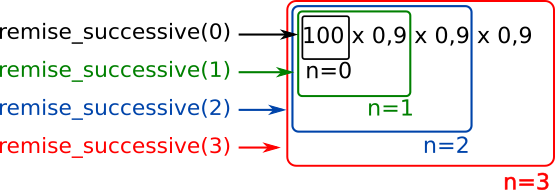
\includegraphics{img/remise_successive.png}
 \end{center}
\end{enumerate}

    \begin{tcolorbox}[breakable, size=fbox, boxrule=1pt, pad at break*=1mm,colback=cellbackground, colframe=cellborder]
\prompt{In}{incolor}{ }{\boxspacing}
\begin{Verbatim}[commandchars=\\\{\}]
\PY{c+c1}{\PYZsh{} 3. et 4.}
\PY{c+c1}{\PYZsh{} Version itérative d\PYZsq{}une remise de 10 \PYZpc{} successives}
\PY{n}{prix} \PY{o}{=} \PY{l+m+mi}{100}
\PY{n}{n}\PY{o}{=}\PY{l+m+mi}{3}
\PY{k}{for} \PY{n}{i} \PY{o+ow}{in} \PY{n+nb}{range}\PY{p}{(}\PY{n}{n}\PY{p}{)}\PY{p}{:}
    \PY{n}{prix} \PY{o}{=} \PY{n}{prix}\PY{o}{*}\PY{p}{(}\PY{l+m+mi}{1}\PY{o}{\PYZhy{}}\PY{l+m+mi}{10}\PY{o}{/}\PY{l+m+mi}{100}\PY{p}{)} \PY{c+c1}{\PYZsh{} prix *= (1\PYZhy{}10/100)}
\PY{n+nb}{print}\PY{p}{(}\PY{n}{prix}\PY{p}{)}
\end{Verbatim}
\end{tcolorbox}

    \begin{tcolorbox}[breakable, size=fbox, boxrule=1pt, pad at break*=1mm,colback=cellbackground, colframe=cellborder]
\prompt{In}{incolor}{1}{\boxspacing}
\begin{Verbatim}[commandchars=\\\{\}]
\PY{c+c1}{\PYZsh{} 5. }
\PY{c+c1}{\PYZsh{} Version récursive}
\PY{k}{def} \PY{n+nf}{remise\PYZus{}successive}\PY{p}{(}\PY{n}{prix}\PY{p}{,}\PY{n}{n}\PY{p}{)}\PY{p}{:}
    \PY{k}{if} \PY{n}{n} \PY{o}{==} \PY{l+m+mi}{0}\PY{p}{:}
        \PY{k}{return} \PY{n}{prix}
    \PY{k}{else}\PY{p}{:}
        \PY{k}{return} \PY{p}{(}\PY{l+m+mi}{1}\PY{o}{\PYZhy{}}\PY{l+m+mi}{10}\PY{o}{/}\PY{l+m+mi}{100}\PY{p}{)}\PY{o}{*}\PY{n}{remise\PYZus{}successive}\PY{p}{(}\PY{n}{prix}\PY{p}{,}\PY{n}{n}\PY{o}{\PYZhy{}}\PY{l+m+mi}{1}\PY{p}{)}

\PY{n+nb}{print}\PY{p}{(}\PY{n}{remise\PYZus{}successive}\PY{p}{(}\PY{l+m+mi}{100}\PY{p}{,}\PY{l+m+mi}{3}\PY{p}{)}\PY{p}{)}
\end{Verbatim}
\end{tcolorbox}

    \begin{Verbatim}[commandchars=\\\{\}]
72.9
    \end{Verbatim}

    \hypertarget{exercice}{%
\subsection*{Exercice}\label{exercice}}

\hypertarget{algorithme-deuclide}{%
\paragraph{Algorithme d'Euclide}\label{algorithme-deuclide}}

L'algorithme d'Euclide permet de trouver le \textbf{plus grand commun
diviseur} de deux nombres entiers positifs \(a\) et \(b\) : on le note
\(PGCD(a;b)\).

Par exemple, le plus grand commun diviseur de \(28\) et \(42\) est
\(14\) que l'on note \(PGCD(28;42)=14\).

    \begin{tcolorbox}[breakable, size=fbox, boxrule=1pt, pad at break*=1mm,colback=cellbackground, colframe=cellborder]
\prompt{In}{incolor}{22}{\boxspacing}
\begin{Verbatim}[commandchars=\\\{\}]
\PY{k}{def} \PY{n+nf}{pgcd}\PY{p}{(}\PY{n}{a}\PY{p}{,}\PY{n}{b}\PY{p}{)}\PY{p}{:}
    \PY{k}{if} \PY{n}{a}\PY{o}{\PYZlt{}}\PY{n}{b}\PY{p}{:}
        \PY{n+nb}{print}\PY{p}{(}\PY{n}{a}\PY{p}{,}\PY{n}{b}\PY{p}{)}
        \PY{n}{a}\PY{p}{,}\PY{n}{b}\PY{o}{=}\PY{n}{b}\PY{p}{,}\PY{n}{a}
        \PY{n+nb}{print}\PY{p}{(}\PY{n}{a}\PY{p}{,}\PY{n}{b}\PY{p}{)}
    \PY{k}{if} \PY{n}{b}\PY{o}{==}\PY{l+m+mi}{0}\PY{p}{:}
        \PY{k}{return} \PY{n}{a}
    \PY{k}{else}\PY{p}{:} 
        \PY{k}{return} \PY{n}{pgcd}\PY{p}{(}\PY{n}{b}\PY{p}{,}\PY{n}{a}\PY{o}{\PYZpc{}}\PY{k}{b})
\end{Verbatim}
\end{tcolorbox}

    \begin{tcolorbox}[breakable, size=fbox, boxrule=1pt, pad at break*=1mm,colback=cellbackground, colframe=cellborder]
\prompt{In}{incolor}{24}{\boxspacing}
\begin{Verbatim}[commandchars=\\\{\}]
\PY{n+nb}{print}\PY{p}{(}\PY{n}{pgcd}\PY{p}{(}\PY{l+m+mi}{280}\PY{p}{,}\PY{l+m+mi}{420}\PY{p}{)}\PY{p}{)}
\end{Verbatim}
\end{tcolorbox}

    \begin{Verbatim}[commandchars=\\\{\}]
280 420
420 280
140
    \end{Verbatim}

    \begin{tcolorbox}[breakable, size=fbox, boxrule=1pt, pad at break*=1mm,colback=cellbackground, colframe=cellborder]
\prompt{In}{incolor}{19}{\boxspacing}
\begin{Verbatim}[commandchars=\\\{\}]
\PY{n}{a}\PY{o}{=}\PY{l+m+mi}{28}
\PY{n}{b}\PY{o}{=}\PY{l+m+mi}{42}
\PY{k}{if} \PY{n}{a}\PY{o}{\PYZlt{}}\PY{n}{b}\PY{p}{:}
    \PY{n}{a}\PY{p}{,}\PY{n}{b}\PY{o}{=}\PY{n}{b}\PY{p}{,}\PY{n}{a}
\PY{n+nb}{print}\PY{p}{(}\PY{n}{a}\PY{p}{,}\PY{n}{b}\PY{p}{)}
\end{Verbatim}
\end{tcolorbox}

    \begin{Verbatim}[commandchars=\\\{\}]
42 28
    \end{Verbatim}

    \begin{tcolorbox}[breakable, size=fbox, boxrule=1pt, pad at break*=1mm,colback=cellbackground, colframe=cellborder]
\prompt{In}{incolor}{18}{\boxspacing}
\begin{Verbatim}[commandchars=\\\{\}]
\PY{l+m+mi}{28}\PY{o}{\PYZpc{}}\PY{k}{14}
\end{Verbatim}
\end{tcolorbox}

            \begin{tcolorbox}[breakable, size=fbox, boxrule=.5pt, pad at break*=1mm, opacityfill=0]
\prompt{Out}{outcolor}{18}{\boxspacing}
\begin{Verbatim}[commandchars=\\\{\}]
0
\end{Verbatim}
\end{tcolorbox}
        
    \hypertarget{exercice}{%
\subsection*{Exercice}\label{exercice}}

\hypertarget{factorielle}{%
\paragraph{Factorielle}\label{factorielle}}

On donne le script de la fonction factorielle à compléter:

\begin{Shaded}
\begin{Highlighting}[]
\KeywordTok{def}\NormalTok{ factorielle(n):}
    \ControlFlowTok{if}\NormalTok{ ...:}
        \ControlFlowTok{return}\NormalTok{ ...}
    \ControlFlowTok{else}\NormalTok{:}
        \ControlFlowTok{return}\NormalTok{ ...}
\end{Highlighting}
\end{Shaded}

    \begin{tcolorbox}[breakable, size=fbox, boxrule=1pt, pad at break*=1mm,colback=cellbackground, colframe=cellborder]
\prompt{In}{incolor}{27}{\boxspacing}
\begin{Verbatim}[commandchars=\\\{\}]
\PY{c+c1}{\PYZsh{} version récursive}

\PY{k}{def} \PY{n+nf}{factorielle}\PY{p}{(}\PY{n}{n}\PY{p}{)}\PY{p}{:}
    \PY{k}{if} \PY{n}{n}\PY{o}{==}\PY{l+m+mi}{1}\PY{p}{:}
        \PY{k}{return} \PY{l+m+mi}{1}
    \PY{k}{else}\PY{p}{:}
        \PY{k}{return} \PY{n}{n}\PY{o}{*}\PY{n}{factorielle}\PY{p}{(}\PY{n}{n}\PY{o}{\PYZhy{}}\PY{l+m+mi}{1}\PY{p}{)}
\end{Verbatim}
\end{tcolorbox}

    \begin{tcolorbox}[breakable, size=fbox, boxrule=1pt, pad at break*=1mm,colback=cellbackground, colframe=cellborder]
\prompt{In}{incolor}{28}{\boxspacing}
\begin{Verbatim}[commandchars=\\\{\}]
\PY{n}{factorielle}\PY{p}{(}\PY{l+m+mi}{5}\PY{p}{)}
\end{Verbatim}
\end{tcolorbox}

            \begin{tcolorbox}[breakable, size=fbox, boxrule=.5pt, pad at break*=1mm, opacityfill=0]
\prompt{Out}{outcolor}{28}{\boxspacing}
\begin{Verbatim}[commandchars=\\\{\}]
120
\end{Verbatim}
\end{tcolorbox}
        
    \begin{tcolorbox}[breakable, size=fbox, boxrule=1pt, pad at break*=1mm,colback=cellbackground, colframe=cellborder]
\prompt{In}{incolor}{1}{\boxspacing}
\begin{Verbatim}[commandchars=\\\{\}]
\PY{c+c1}{\PYZsh{} version itérative avec while}

\PY{k}{def} \PY{n+nf}{factorielle}\PY{p}{(}\PY{n}{n}\PY{p}{)}\PY{p}{:}
    \PY{n}{p} \PY{o}{=} \PY{l+m+mi}{1}
    \PY{k}{while} \PY{n}{n}\PY{o}{\PYZgt{}}\PY{l+m+mi}{0}\PY{p}{:}
        \PY{n}{p} \PY{o}{*}\PY{o}{=} \PY{n}{n} \PY{c+c1}{\PYZsh{} p = p * n}
        \PY{n}{n} \PY{o}{\PYZhy{}}\PY{o}{=} \PY{l+m+mi}{1} \PY{c+c1}{\PYZsh{} n = n\PYZhy{}1}
    \PY{k}{return} \PY{n}{p}

\PY{n}{factorielle}\PY{p}{(}\PY{l+m+mi}{5}\PY{p}{)}
\end{Verbatim}
\end{tcolorbox}

            \begin{tcolorbox}[breakable, size=fbox, boxrule=.5pt, pad at break*=1mm, opacityfill=0]
\prompt{Out}{outcolor}{1}{\boxspacing}
\begin{Verbatim}[commandchars=\\\{\}]
120
\end{Verbatim}
\end{tcolorbox}
        
    \begin{tcolorbox}[breakable, size=fbox, boxrule=1pt, pad at break*=1mm,colback=cellbackground, colframe=cellborder]
\prompt{In}{incolor}{2}{\boxspacing}
\begin{Verbatim}[commandchars=\\\{\}]
\PY{c+c1}{\PYZsh{} version itérative avec for}

\PY{k}{def} \PY{n+nf}{factorielle}\PY{p}{(}\PY{n}{n}\PY{p}{)}\PY{p}{:}
    \PY{n}{p} \PY{o}{=} \PY{l+m+mi}{1}
    \PY{k}{for} \PY{n}{i} \PY{o+ow}{in} \PY{n+nb}{range}\PY{p}{(}\PY{l+m+mi}{1}\PY{p}{,}\PY{n}{n}\PY{o}{+}\PY{l+m+mi}{1}\PY{p}{)}\PY{p}{:}
        \PY{n}{p} \PY{o}{*}\PY{o}{=} \PY{n}{i} \PY{c+c1}{\PYZsh{} p = p * i}
    \PY{k}{return} \PY{n}{p}

\PY{n}{factorielle}\PY{p}{(}\PY{l+m+mi}{5}\PY{p}{)}
\end{Verbatim}
\end{tcolorbox}

            \begin{tcolorbox}[breakable, size=fbox, boxrule=.5pt, pad at break*=1mm, opacityfill=0]
\prompt{Out}{outcolor}{2}{\boxspacing}
\begin{Verbatim}[commandchars=\\\{\}]
120
\end{Verbatim}
\end{tcolorbox}
        
    \hypertarget{exercice}{%
\subsection*{Exercice}\label{exercice}}

Dessin récursif avec Turtle à réaliser sur Thonny ou autre idle Python.

    \begin{tcolorbox}[breakable, size=fbox, boxrule=1pt, pad at break*=1mm,colback=cellbackground, colframe=cellborder]
\prompt{In}{incolor}{1}{\boxspacing}
\begin{Verbatim}[commandchars=\\\{\}]
\PY{k+kn}{from} \PY{n+nn}{turtle} \PY{k+kn}{import} \PY{o}{*}

\PY{n}{couleurs}\PY{o}{=}\PY{p}{[}\PY{l+s+s1}{\PYZsq{}}\PY{l+s+s1}{blue}\PY{l+s+s1}{\PYZsq{}}\PY{p}{,}\PY{l+s+s1}{\PYZsq{}}\PY{l+s+s1}{green}\PY{l+s+s1}{\PYZsq{}}\PY{p}{,}\PY{l+s+s1}{\PYZsq{}}\PY{l+s+s1}{yellow}\PY{l+s+s1}{\PYZsq{}}\PY{p}{,}\PY{l+s+s1}{\PYZsq{}}\PY{l+s+s1}{orange}\PY{l+s+s1}{\PYZsq{}}\PY{p}{,}\PY{l+s+s1}{\PYZsq{}}\PY{l+s+s1}{red}\PY{l+s+s1}{\PYZsq{}}\PY{p}{,}\PY{l+s+s1}{\PYZsq{}}\PY{l+s+s1}{purple}\PY{l+s+s1}{\PYZsq{}}\PY{p}{]}
\PY{n}{bgcolor}\PY{p}{(}\PY{l+s+s1}{\PYZsq{}}\PY{l+s+s1}{black}\PY{l+s+s1}{\PYZsq{}}\PY{p}{)}

\PY{k}{def} \PY{n+nf}{dessin}\PY{p}{(}\PY{p}{)}\PY{p}{:}
    \PY{k}{for} \PY{n}{i} \PY{o+ow}{in} \PY{n+nb}{range}\PY{p}{(}\PY{l+m+mi}{180}\PY{p}{)}\PY{p}{:}
        \PY{n}{color}\PY{p}{(}\PY{n}{couleurs}\PY{p}{[}\PY{n}{i}\PY{o}{\PYZpc{}}\PY{k}{6}])
        \PY{n}{forward}\PY{p}{(}\PY{n}{i}\PY{p}{)}
        \PY{n}{right}\PY{p}{(}\PY{l+m+mi}{59}\PY{p}{)}
        
\PY{n}{dessin}\PY{p}{(}\PY{p}{)}
\end{Verbatim}
\end{tcolorbox}

    \hypertarget{exercice}{%
\subsection*{Exercice}\label{exercice}}

Calcul récursif d'une puissance.

    \begin{tcolorbox}[breakable, size=fbox, boxrule=1pt, pad at break*=1mm,colback=cellbackground, colframe=cellborder]
\prompt{In}{incolor}{18}{\boxspacing}
\begin{Verbatim}[commandchars=\\\{\}]
\PY{k}{def} \PY{n+nf}{puissance}\PY{p}{(}\PY{n}{x}\PY{p}{,}\PY{n}{n}\PY{p}{)}\PY{p}{:}
    \PY{k}{if} \PY{n}{n}\PY{o}{==}\PY{l+m+mi}{0}\PY{p}{:}
        \PY{k}{return} \PY{l+m+mi}{1}
    \PY{k}{else}\PY{p}{:}
        \PY{c+c1}{\PYZsh{}print(x,n)}
        \PY{k}{return} \PY{n}{x}\PY{o}{*}\PY{n}{puissance}\PY{p}{(}\PY{n}{x}\PY{p}{,}\PY{n}{n}\PY{o}{\PYZhy{}}\PY{l+m+mi}{1}\PY{p}{)}
\end{Verbatim}
\end{tcolorbox}

    \begin{tcolorbox}[breakable, size=fbox, boxrule=1pt, pad at break*=1mm,colback=cellbackground, colframe=cellborder]
\prompt{In}{incolor}{21}{\boxspacing}
\begin{Verbatim}[commandchars=\\\{\}]
\PY{n}{puissance}\PY{p}{(}\PY{l+m+mi}{3}\PY{p}{,}\PY{l+m+mi}{7}\PY{p}{)}
\end{Verbatim}
\end{tcolorbox}

    \begin{Verbatim}[commandchars=\\\{\}]
3 7
3 6
3 5
3 4
3 3
3 2
3 1
    \end{Verbatim}

            \begin{tcolorbox}[breakable, size=fbox, boxrule=.5pt, pad at break*=1mm, opacityfill=0]
\prompt{Out}{outcolor}{21}{\boxspacing}
\begin{Verbatim}[commandchars=\\\{\}]
2187
\end{Verbatim}
\end{tcolorbox}
        
    \begin{tcolorbox}[breakable, size=fbox, boxrule=1pt, pad at break*=1mm,colback=cellbackground, colframe=cellborder]
\prompt{In}{incolor}{20}{\boxspacing}
\begin{Verbatim}[commandchars=\\\{\}]
\PY{l+s+sd}{\PYZdq{}\PYZdq{}\PYZdq{}}
\PY{l+s+sd}{On peut améliorer l\PYZsq{}algorithme des puissances en regardant la parité de l\PYZsq{}exposant.}
\PY{l+s+sd}{\PYZhy{} si n est pair, alors n=2p et x**n = (x**2)**p}
\PY{l+s+sd}{\PYZhy{} si n est impair, alors n=2p+1 et x**n = x(x**2)**p}

\PY{l+s+sd}{Exemple:}
\PY{l+s+sd}{\PYZhy{} x**12 = (x**2)**6 = ((x**2)**2)**3 = ((x**2)**2)**2)x }
\PY{l+s+sd}{soit 4 appels de la fonction au lieu de 12 avec la version classique.}

\PY{l+s+sd}{\PYZhy{} x**8 = (x**2)**4 = ((x**2)**2)**2}
\PY{l+s+sd}{soit 3 appels de la fonction au lieu de 8 avec la version classique.}

\PY{l+s+sd}{Remarque: pour un exposant égal à n=256, il y aura 256 appels récursifs avec la première version }
\PY{l+s+sd}{contre seulement 8 avec la seconde. En plus des appels récursifs, ce sont nettement moins de calculs !}
\PY{l+s+sd}{\PYZdq{}\PYZdq{}\PYZdq{}}

\PY{k}{def} \PY{n+nf}{puissance2}\PY{p}{(}\PY{n}{x}\PY{p}{,}\PY{n}{n}\PY{p}{)}\PY{p}{:}
    \PY{k}{if} \PY{n}{n}\PY{o}{==}\PY{l+m+mi}{1}\PY{p}{:}
        \PY{k}{return} \PY{n}{x}
    \PY{k}{else}\PY{p}{:}
        \PY{c+c1}{\PYZsh{}print(x,n)}
        \PY{k}{if} \PY{n}{n}\PY{o}{\PYZpc{}}\PY{k}{2}==0:
            \PY{k}{return} \PY{n}{puissance2}\PY{p}{(}\PY{n}{x}\PY{o}{*}\PY{o}{*}\PY{l+m+mi}{2}\PY{p}{,}\PY{n}{n}\PY{o}{/}\PY{o}{/}\PY{l+m+mi}{2}\PY{p}{)}
        \PY{k}{else}\PY{p}{:}
            \PY{k}{return} \PY{n}{x}\PY{o}{*}\PY{n}{puissance2}\PY{p}{(}\PY{n}{x}\PY{o}{*}\PY{o}{*}\PY{l+m+mi}{2}\PY{p}{,}\PY{n}{n}\PY{o}{/}\PY{o}{/}\PY{l+m+mi}{2}\PY{p}{)}
\end{Verbatim}
\end{tcolorbox}

    \begin{tcolorbox}[breakable, size=fbox, boxrule=1pt, pad at break*=1mm,colback=cellbackground, colframe=cellborder]
\prompt{In}{incolor}{14}{\boxspacing}
\begin{Verbatim}[commandchars=\\\{\}]
\PY{n}{puissance2}\PY{p}{(}\PY{l+m+mi}{3}\PY{p}{,}\PY{l+m+mi}{256}\PY{p}{)}
\end{Verbatim}
\end{tcolorbox}

    \begin{Verbatim}[commandchars=\\\{\}]
3 256
9 128
81 64
6561 32
43046721 16
1853020188851841 8
3433683820292512484657849089281 4
11790184577738583171520872861412518665678211592275841109096961 2
    \end{Verbatim}

            \begin{tcolorbox}[breakable, size=fbox, boxrule=.5pt, pad at break*=1mm, opacityfill=0]
\prompt{Out}{outcolor}{14}{\boxspacing}
\begin{Verbatim}[commandchars=\\\{\}]
13900845237714473276493978678966130311421885080852913799160482443003607262976643
5941001769154109609521811665540548899435521
\end{Verbatim}
\end{tcolorbox}
        
    \hypertarget{exercice}{%
\subsection*{Exercice}\label{exercice}}

\hypertarget{algorithme-mystuxe8re}{%
\paragraph{Algorithme mystère}\label{algorithme-mystuxe8re}}

    \begin{tcolorbox}[breakable, size=fbox, boxrule=1pt, pad at break*=1mm,colback=cellbackground, colframe=cellborder]
\prompt{In}{incolor}{3}{\boxspacing}
\begin{Verbatim}[commandchars=\\\{\}]
\PY{k}{def} \PY{n+nf}{mystere}\PY{p}{(}\PY{n}{n}\PY{p}{)}\PY{p}{:}
    \PY{k}{if} \PY{n}{n}\PY{o}{\PYZlt{}}\PY{l+m+mi}{2}\PY{p}{:}
        \PY{k}{return} \PY{n+nb}{str}\PY{p}{(}\PY{n}{n}\PY{p}{)}
    \PY{k}{else}\PY{p}{:}
        \PY{k}{return} \PY{n}{mystere}\PY{p}{(}\PY{n}{n}\PY{o}{/}\PY{o}{/}\PY{l+m+mi}{2}\PY{p}{)}\PY{o}{+}\PY{n+nb}{str}\PY{p}{(}\PY{n}{n}\PY{o}{\PYZpc{}}\PY{k}{2})
\end{Verbatim}
\end{tcolorbox}

    \begin{tcolorbox}[breakable, size=fbox, boxrule=1pt, pad at break*=1mm,colback=cellbackground, colframe=cellborder]
\prompt{In}{incolor}{4}{\boxspacing}
\begin{Verbatim}[commandchars=\\\{\}]
\PY{n}{mystere}\PY{p}{(}\PY{l+m+mi}{10}\PY{p}{)}
\end{Verbatim}
\end{tcolorbox}

            \begin{tcolorbox}[breakable, size=fbox, boxrule=.5pt, pad at break*=1mm, opacityfill=0]
\prompt{Out}{outcolor}{4}{\boxspacing}
\begin{Verbatim}[commandchars=\\\{\}]
'1010'
\end{Verbatim}
\end{tcolorbox}
        
    \hypertarget{compluxe9ment-uxe0-2}{%
\subsection*{Complément à 2}\label{compluxe9ment-uxe0-2}}

En première, on a vu l'écriture binaire des nombres signés pour les
nombres entiers relatifs.

On rappelle qu'un nombre signé positif a son bit de poids fort égal à 0
et un nombre négatif a son bit de poids fort égal à 1.

\hypertarget{muxe9thode-1uxe8re}{%
\paragraph{Méthode (1ère)}\label{muxe9thode-1uxe8re}}

La méthode consite à : - donner l'écriture binaire de la valeur absolue
du nombre - donner le complément à 1 de cette écriture binaire, - puis
le complément à 2 en ajoutant 1 au complément à 1.

La méthode du complément à 2 se généralise de la façon suivante:
\#\#\#\# Propriété: Soit \textbf{n} le nombre de bits utilisés pour
coder les entiers relatifs. On peut coder tous les nombres compris entre
\(-2^{n-1}\) et \(2^{n-1}-1\).

\hypertarget{exemple}{%
\subparagraph{Exemple}\label{exemple}}

Par exemple, sur \(n=4\) bits, on peut coder les entiers compris entre
\(-2^{3}=-8\) et \(2^{n-1}-1=8-1=7\)

\hypertarget{muxe9thode}{%
\paragraph{Méthode}\label{muxe9thode}}

Pour coder un nombre r entier relatif : - il faut déterminer le nombre
minimal de bits à utiliser, - si r est positif, on le code en binaire -
si r est négatif, on code le nombre \(r+2^{n}\)

\hypertarget{exemple-1}{%
\subparagraph{Exemple}\label{exemple-1}}

Écriture binaire de -5

On a : \(-8<-5<7\) ce qui est équivalent à \(-2^{3} < -5 < 2^{3}-1\)\\
On en déduit que \(n=4\) bits. L'écriture binaire de \(-5\) est la même
que son complément à \(2^{4}\) soit \(-5+2^{4}=11\)\\
Or \(11_{10}=1011_{2}\) donc \(-5_{10}=1011_{2}\)

    \begin{tcolorbox}[breakable, size=fbox, boxrule=1pt, pad at break*=1mm,colback=cellbackground, colframe=cellborder]
\prompt{In}{incolor}{5}{\boxspacing}
\begin{Verbatim}[commandchars=\\\{\}]
\PY{k}{def} \PY{n+nf}{binaire}\PY{p}{(}\PY{n}{r}\PY{p}{,}\PY{n}{n}\PY{p}{)}\PY{p}{:}
    \PY{k}{if} \PY{n}{r}\PY{o}{\PYZgt{}}\PY{o}{=}\PY{l+m+mi}{0}\PY{p}{:}
        \PY{k}{return} \PY{n}{mystere}\PY{p}{(}\PY{n}{n}\PY{p}{)}
    \PY{k}{else}\PY{p}{:}
        \PY{k}{return} \PY{n}{mystere}\PY{p}{(}\PY{n}{r}\PY{o}{+}\PY{l+m+mi}{2}\PY{o}{*}\PY{o}{*}\PY{n}{n}\PY{p}{)}
\end{Verbatim}
\end{tcolorbox}

    \begin{tcolorbox}[breakable, size=fbox, boxrule=1pt, pad at break*=1mm,colback=cellbackground, colframe=cellborder]
\prompt{In}{incolor}{8}{\boxspacing}
\begin{Verbatim}[commandchars=\\\{\}]
\PY{c+c1}{\PYZsh{} 2\PYZca{}5=32 et 2\PYZca{}6=64}
\PY{c+c1}{\PYZsh{} on a \PYZhy{}64 \PYZlt{} \PYZhy{}35 \PYZlt{} 63 donc \PYZhy{}2\PYZca{}6 \PYZlt{} \PYZhy{}35 \PYZlt{} 2\PYZca{}6\PYZhy{}1 donc n=7 bits}
\PY{n}{binaire}\PY{p}{(}\PY{o}{\PYZhy{}}\PY{l+m+mi}{35}\PY{p}{,}\PY{l+m+mi}{7}\PY{p}{)}
\end{Verbatim}
\end{tcolorbox}

            \begin{tcolorbox}[breakable, size=fbox, boxrule=.5pt, pad at break*=1mm, opacityfill=0]
\prompt{Out}{outcolor}{8}{\boxspacing}
\begin{Verbatim}[commandchars=\\\{\}]
'1011101'
\end{Verbatim}
\end{tcolorbox}
        
    \hypertarget{exercice}{%
\subsection*{Exercice}\label{exercice}}

\hypertarget{suite-de-fibonacci}{%
\paragraph{Suite de Fibonacci}\label{suite-de-fibonacci}}

La suite de fibonacci se construit par addition des deux nombres
précédents: Les deux premiers nombres étant 0 et 1.

Donc : 0,1,1,2,3,5,8,13,21,34,etc.

    \begin{tcolorbox}[breakable, size=fbox, boxrule=1pt, pad at break*=1mm,colback=cellbackground, colframe=cellborder]
\prompt{In}{incolor}{5}{\boxspacing}
\begin{Verbatim}[commandchars=\\\{\}]
\PY{k}{def} \PY{n+nf}{fibonacci}\PY{p}{(}\PY{n}{n}\PY{p}{)}\PY{p}{:}
    \PY{k}{if} \PY{n}{n}\PY{o}{==}\PY{l+m+mi}{0}\PY{p}{:}
        \PY{k}{return} \PY{l+m+mi}{0}
    \PY{k}{elif} \PY{n}{n}\PY{o}{==}\PY{l+m+mi}{1}\PY{p}{:}
        \PY{k}{return} \PY{l+m+mi}{1}
    \PY{k}{else}\PY{p}{:}
        \PY{k}{return} \PY{n}{fibonacci}\PY{p}{(}\PY{n}{n}\PY{o}{\PYZhy{}}\PY{l+m+mi}{2}\PY{p}{)}\PY{o}{+}\PY{n}{fibonacci}\PY{p}{(}\PY{n}{n}\PY{o}{\PYZhy{}}\PY{l+m+mi}{1}\PY{p}{)}
\end{Verbatim}
\end{tcolorbox}

    \begin{tcolorbox}[breakable, size=fbox, boxrule=1pt, pad at break*=1mm,colback=cellbackground, colframe=cellborder]
\prompt{In}{incolor}{6}{\boxspacing}
\begin{Verbatim}[commandchars=\\\{\}]
\PY{k}{for} \PY{n}{i} \PY{o+ow}{in} \PY{n+nb}{range}\PY{p}{(}\PY{l+m+mi}{20}\PY{p}{)}\PY{p}{:}
    \PY{n+nb}{print}\PY{p}{(}\PY{n}{fibonacci}\PY{p}{(}\PY{n}{i}\PY{p}{)}\PY{p}{)}
\end{Verbatim}
\end{tcolorbox}

    \begin{Verbatim}[commandchars=\\\{\}]
0
1
1
2
3
5
8
13
21
34
55
89
144
233
377
610
987
1597
2584
4181
    \end{Verbatim}

   
    
    
\end{document}
